
\chapter[Contratações de Fornecedores de Desenvolvimento de Software]{Contratações de Fornecedores de Desenvolvimento de Software}

O descumprimento da legislação de licitações e contratos gera riscos para a contratação de tecnologia da informação e, portanto, devem ser conhecidos e usados como base de qualquer processo de contratação de fornecedores de desenvolvimento de \textit{software}. Assim, neste capítulo será apresentada uma visão sobre a importância da contratação de serviços de TI e a caracterização de contratação de tecnologia da informação pelas organizações públicas brasileiras, segundo a legislação pertinente, apresentando-se, de forma resumida, os conceitos de contratação de serviços de TI presentes em normas, modelos, guias e processos de contratação de soluções de TI.

\section[Importância da Contração de Fornecedores de Desenvolvimento de Software]{Importância da Contração de Fornecedores de Desenvolvimento de Software}

Um dos atos administrativos principais, mais complexos e mais frequentemente utilizados é a contratação. Contratar é fazer contrato, que é um acordo ou convenção entre duas ou mais pessoas para a execução de alguma coisa, sob determinadas condições. O contrato é, portanto, o documento em que se registra esse acordo ou convenção \cite{MPOG:2011}.

Há vários anos, os órgãos da Administração Pública Federal (APF) têm adotado a prática da execução indireta de muitos serviços que dão suporte às suas áreas-fim, conhecida comumente como “terceirização de serviços”. O Decreto-Lei 200/1967 traz, no Art.10 § 7º, a diretriz para que a Administração Pública Federal se desobrigue da realização de tarefas executivas (execução de tarefas operacionais), recorrendo, sempre que possível, à execução indireta, desde que a iniciativa privada esteja suficientemente desenvolvida na área, bem como não haja comprometimento da segurança nacional (Art.10 §8º). De acordo com o Decreto-Lei 200/1967, Art.10, §7º, as razões para se partir para execução indireta são: possibilitar que a APF execute melhor as tarefas de planejamento, coordenação, supervisão e controle, tarefas que hoje podem ser traduzidas como gestão e governança; impedir o crescimento desmesurado da máquina administrativa, para que o Estado não alcance dimensão indevida em função da incorporação de tarefas de caráter operacional  \cite{TCU:2012}. 

Um levantamento do Tribunal de Contas da União (TCU) mostrou que o orçamento de gastos em TI da Administração Pública Federal de 2010 era de pelo menos 12,5 bilhões de reais, sendo grande parte desse valor destinado a contratações de serviços relacionados a \textit{software}. No mesmo ano, também era previsto um orçamento de cerca de 1,8 trilhão de reais da União, sendo que a maior parte seria gasto em TI. Com isso, os serviços de TI requerem bastante atenção e tem suma importância para administração pública brasileira, tanto no que diz respeito a contratações ou desenvolvimento de produtos de TI.

A definição e institucionalização de processos de contratação de serviços de TI, especialmente aqueles relacionados a \textit{software}, envolvem ações complexas, principalmente no que diz respeito à identificação dos requisitos necessários, a garantia da qualidade dos resultados esperados, aos critérios de aceitação, a gestão de mudanças, as transferências de conhecimentos, a legislação pertinente, entre outros. Envolvem também questões de relacionamento entre clientes e fornecedores, o que implica em competências administrativas e jurídicas. Essas complexidades apresentam riscos para partes envolvidas e, como consequência, é comum a ocorrência de conflitos \cite{cruz2011}.

Assim, contratações envolvem riscos e incertezas oriundos de diversos fatores inerentes do objeto do contrato. Com isso, é preciso observar as características do objeto e do contexto em que ele será inserido, com especial atenção à conformidade legal em contratações de serviços de TI em organizações públicas, para que seja realizado o devido controle.


\section[Normas, Processos e Legislação Pertinentes à Contratação]{Normas, Processos e Legislação Pertinentes à Contratação}

\subsection[Lei nº 8.666/93]{Lei nº 8.666/93}

A Lei nº 8.666 \cite{Lei8666:1993} estabelece normas gerais sobre licitações e contratos administrativos. A licitação é tida como antecedente ao contrato administrativo e pode ser considerado o procedimento no qual a Administração Pública escolhe a proposta mais vantajosa para contrato do seu interesse e, ao mesmo tempo, dá igual oportunidade aos que desejam fazer parte do contrato.

Uma licitação supõe concorrência entre ofertantes, portanto, os objetos propensos à licitação são aqueles que podem ser fornecidos por mais uma pessoa ou entidade. Os princípios da licitação de acordo com o Art. 3º são:
\begin{itemize}
\item Igualdade: é impedida a existência de cláusulas no edital que favorecem um em detrimento de outros, mas não é considerado atentado ao princípio da igualdade estabelecer requisitos mínimos de participação;
\item Legalidade: a licitação é um procedimento completamente vinculado à lei;
\item Impessoalidade: a Administração deve considerar critérios claros e objetivos para a escolha do licitante, todos devem ser tratados igualmente em termos de direito e obrigações;
\item Moralidade e Probidade Administrativa: é passível de punição qualquer comportamento que vá contra a moral, bons costumes, as regras de boa administração e aos princípios de justiça e equidade;
\item Publicidade: diz respeito tanto à divulgação da licitação para todos os interessados como também a todos os atos praticados pela Administração durante as fases, para que sejam abertos aos interessados;
\item Vinculação ao Instrumento Convocatório: o edital deve estar vinculado à licitação e sua alteração só é permitida quando for falho ou inadequado ao interesse público;
\item Julgamento Objetivo: diz respeito a utilizar o critério indicado no ato convocatório para julgamento das propostas, seja ela técnica ou de preço;
\item Fiscalização da Licitação: qualquer cidadão poder controlar a licitação contra irregularidades na aplicação da lei;
\item Competitividade: a lei proíbe a existência de cláusulas que vão contra o caráter competitivo da licitação, salvo os casos de só haver um interessado ou um concorrente após a fase de classificação;
\item Padronização: sempre que possível, deve ser adotada a padronização.
\end{itemize}

A licitação pode ser classificada quanto a modalidade, que está relacionada ao valor estimado do contrato, ou ao tipo, que está relacionado ao julgamento. A Lei nº 8.666 prevê cinco modalidades de licitação no Art. 22: concorrência, tomada de preços, convite, concurso e leilão. As modalidades sem finalidade específica entram no grupo formado pela concorrência, pela tomada de preços e pelo convite. O grupo das modalidades com finalidades específicas é formado pelo concurso e pelo leilão. Os quatro tipos de licitação presentes no Art.45 são: 
\begin{itemize}
\item Menor preço: aquela em que o fator de decisão é apenas o menor preço e as demais características, como qualidade e produtividade, não são consideradas;
\item Melhor técnica: não considera só o preço, mas as melhores tecnologias, aquelas mais modernas ou que satisfaçam da melhor forma as necessidades da Administração licitante e que estejam dentro dos recursos financeiros disponíveis;
\item Técnica e preço: aquela em que é feita uma ponderação para técnica e preço a fim de considerar ambos;
\item Maior lance ou oferta: é escolhida a proposta que faz a maior oferta, este tipo é especialmente usado em vendas de bens ou permissões de uso de bens ou serviços públicos.
\end{itemize}

Uma licitação é constituída por fases, sendo elas: interna (destinada a firmar a intenção da entidade licitante e obter informações necessárias para a consolidação da licitação); e a externa (destinada a selecionar a melhor proposta). A fase interna é composta por determinar o objeto de licitação, as condições, a estimativa de despesas e a decisão pela modalidade mais adequada, além da verificação da existência de recursos e a obtenção da autorização de abertura do instrumento convocatório.

Já a fase externa é dividida de forma geral em: abertura, habilitação, classificação e julgamento.  A abertura é o momento em que o instrumento convocatório, edital ou carta-convite, é tornado conhecido publicamente; a habilitação é onde a comissão de licitação confirma os licitantes aptos a participarem da licitação de acordo com o edital; a classificação é o ato no qual a comissão de licitação reúne as propostas apresentadas formalmente e, de acordo com o edital ou carta-convite, que são aptas ou não para classificação; o julgamento costuma ocorrer logo após a classificação das propostas e é considerado apenas o que foi permitido no instrumento convocatório, feito de acordo com um dos quatro tipos de licitação, previsto no edital. 

Após o julgamento, é realizado o processo de homologação e adjudicação. Na homologação, uma autoridade competente, indicada por lei, promove o controle de todo processo licitatório no que diz respeito à legalidade, e na adjudicação, é atribuído ao vencedor o objeto da licitação pela mesma autoridade competente. Outros detalhes da Lei nº 8.666 não foram considerados pertinentes para o escopo deste trabalho.


\subsection[Instrução Normativa nº 04]{Instrução Normativa nº 04}

A Instrução Normativa nº 04 \cite{IN04:2010}, disciplina sobre o processo de Contratação de Soluções de Tecnologia da Informação pelos órgãos integrantes do Sistema de Administração dos Recursos de Informação e Informática do Poder  Executivo Federal, é a consolidação de um conjunto de boas práticas para Contratação de Solução de TI pela Administração Pública Federal. Este conjunto de boas práticas é chamado de Modelo de Contratações de Soluções de TI (MCTI). Esta Instrução Normativa está dividida em três capítulos: o primeiro diz respeito às Disposições Gerais; o segundo, fala do Processo de Contratação; e o terceiro nos apresenta as Disposições Finais - este não será detalhado, pois não faz parte do escopo deste trabalho.

\subsubsection[Disposições Gerais]{Disposições Gerais}

De forma geral, no capítulo das Disposições Gerais é mencionado os atores, os artefatos e o que é vedado no processo de contratações. Estes, de acordo com Art. 2º, são: 

\begin{itemize}
\item Área requisitante da solução: entidade ou órgão que demanda a contratação de uma Solução de Tecnologia da Informação; 
\item Área de tecnologia da informação: unidade setorial do SISP responsável por gerir a Tecnologia da Informação do órgão ou entidade;
\item Equipe de planejamento da contratação: constituída pelo integrante técnico (servidor da área de TI), integrante administrativo (servidor da área administrativa) e integrante requisitante (servidor da área requisitante);
\item Gestor do contrato: servidor com atribuições gerenciais, técnicas e operacionais responsável pela gestão do contrato; 
\item Fiscal técnico do contrato: servidor da área de TI; 
\item Fiscal administrativo do contrato: servidor da área administrativa; 
\item Fiscal requisitante do contrato: servidor da área requisitante;
\item Contratada: entidade provedora da Solução de Tecnologia da Informação;
\item Preposto: funcionário representante da contratada, responsável por acompanhar a execução do contrato e atuar como interlocutor principal junto à contratante.
\end{itemize}

Os artefatos que podem ser produzidos e fornecidos para a contratada ou recebidos pelo contratante são: a solução de tecnologia da informação; os requisitos; o documento de oficialização da demanda; a análise de viabilidade da contratação; o plano de sustentação; a estratégia da contratação; a análise de riscos; o plano de inserção; a ordem de serviço ou de fornecimento de bens; o termo de recebimento provisório; o termo de recebimento definitivo; os critérios de aceitação; a gestão e o plano diretor de tecnologia da informação.

Nas Disposições Gerais, é ressaltado, no Art.5º, que não poderão ser objeto de contratação mais de uma solução de TI em um único contrato e a gestão de processos de TI.  No Art. 6º é dito que a contratada que provê a solução de TI não poderá ser a mesma que realiza medições, avaliação ou fiscalização e é vedado, segundo o Art. 7º, prever a remuneração dos funcionários da contratada já no edital, reembolsar despesas que são de exclusiva responsabilidade da contratada, exigir qualquer tipo de capacitação ou certificação no edital, demandar aos funcionários da contratada tarefas fora do escopo do objetivo da contratação e indicar pessoas para compor o quadro funcional da contratada. 

Está presente, ainda nas Disposições Gerais, a Estratégia Geral de Tecnologia da Informação (EGTI), que contém orientações gerais para as áreas de TI e dos órgãos e entidades da Administração Pública, Federação e a formulação de um Plano Diretor de Tecnologia da Informação (PDTI) por parte de cada entidade integrante do Sistema de Administração dos Recursos de Informação e Informática (SISP) do Poder Executivo Federal. De forma geral, neste documento, são apresentados a avaliação e o diagnóstico dos recursos de TI, as necessidades da entidade e o planejamento de investimentos e recursos.

\subsubsection[Processo de Contratação]{Processo de Contratação}

O Processo de Contratação é, de fato, o MCTI (Fig. \ref{mcti}), que divide as contratações de soluções de TI em três fases: Planejamento da Contratação (PCTI); Seleção do Fornecedor (SFTI) e Gerenciamento do Contrato (GCTI).

\begin{figure}[h]
		\centering
		\label{fig05}
			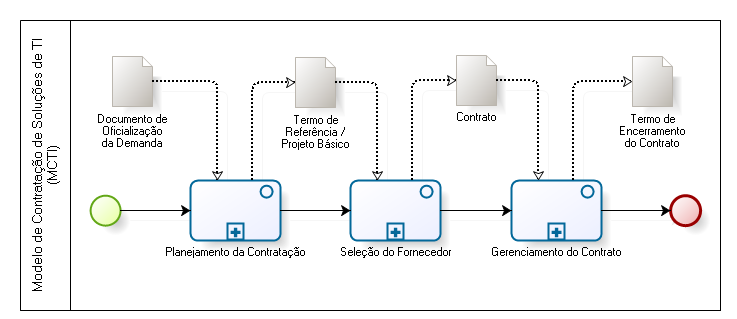
\includegraphics[scale=0.8]{figuras/MCTI.png}
		\caption{Modelo de Contratações de Soluções de TI   \cite{mcti}}
\label{mcti}
\end{figure}


Cada fase é constituída de processos/etapas, atividades, artefatos e atores, conforme mostrado na Tab. (\ref{fmcti}).
  
\begin{table}[htb]
\center
\footnotesize
\begin{tabular}{|p{1.4cm}|p{1cm}|p{3cm}|p{3cm}|p{3cm}|}
  \hline
   \textbf{Fases} & \textbf{Etapas}  & \textbf{Atividades}  & \textbf{Artefatos} & \textbf{Atores}  \\
    \hline
    PCTI & 5 & 41 & 8 & 7\\
   \hline    
    SFTI & 3 & 7 & 1 & 4\\
    \hline
    GCTI & 5 & 19 & 4 & 5\\
   \hline
\end{tabular}
\caption{Fases do MCTI}
\label{fmcti}
\end{table}

\textbf {Planejamento da Contratação}

No Planejamento da Contratação é necessário ter, no mínimo, o documento mostrando quais são as necessidades corporativas da instituição e seus objetivos estratégicos, motivação, resultados esperados, fonte de recursos e a indicação do integrante requisitante que fará parte da equipe de planejamento.  Após o recebimento desse documento, a área de TI indicará o integrante técnico que também fará parte da equipe de planejamento e, então, finalmente, o documento será encaminhado para a área administrativa, que indicará o integrante administrativo que fará parte da equipe de planejamento e dará prosseguimento para a contratação. Assim, a equipe estará completa para acompanhar e apoiar todas as atividades presentes nas fases de planejamento de contratação e seleção do fornecedor.

A fase de Planejamento da Contratação é obrigatória. Independentemente do tipo de contratação, deve ser elaborada em harmonia com o PDTI e contém cinco etapas: 
\begin{itemize}
\item Análise de viabilidade; 
\item Plano de sustentação; 
\item Estratégia da contratação; 
\item Análise de riscos; 
\item Termo de referência ou projeto básico.
\end{itemize}

A análise de viabilidade da contratação compreende a definição e a especificação de requisitos, levando em conta que compete ao integrante técnico especificar os requisitos tecnológicos, e ao integrante requisitante os demais requisitos, a identificação de possíveis soluções, análise e comparação de custos totais dessas soluções, a escolha da solução de TI e a justificativa da solução escolhida e avaliação das necessidades de adequação para viabilização da execução contratual. 

O plano de sustentação deve conter quais os recursos materiais e humanos que serão necessários, atividades de transição contratual e encerramento do contrato, assim como a continuidade do fornecimento da solução de TI em caso de interrupção contratual e a estratégia de independência do contratante com relação à contratada. 

A estratégia da contratação será elaborada a partir das duas etapas anteriores e conterá a indicação da solução de TI a ser contratada. A definição das responsabilidades da contratada, além das estabelecidas no contrato, é: a indicação dos termos contratuais, observando os elementos contidos na Lei nº 8.666, de 1993, a elaboração do orçamento detalhado, da estimativa do impacto econômico-financeiro no orçamento do órgão requisitante, a elaboração dos termos de compromisso e sigilo e a definição dos critérios técnicos de julgamento das propostas para a fase de seleção de fornecedor. 

A análise de riscos deverá conter identificação dos principais riscos que podem comprometer o sucesso dos processos de contratação e de gestão contratual ou que possam fazer com que a solução de TI não atenda às necessidades esperadas, a mensuração das probabilidades de ocorrência e dos dados potenciais relacionados a cada risco, a definição das ações de contingência em caso de ocorrência dos ricos e a definição dos responsáveis pelas ações de prevenção e de contingência dos riscos.

O termo de referência ou projeto básico deverá conter, no mínimo, a definição do objetivo, a fundamentação da contratação, a descrição da solução de TI, os requisitos da solução, o modelo de prestação de serviços ou de fornecimento de bens, os elementos para gestão do contrato, a estimativa de preços, a adequação orçamentária, as definições dos critérios de sanções e os critérios de seleção do fornecedor. 

\textbf {Seleção do Fornecedor}

Na fase de Seleção de Fornecedor, são observadas as normas pertinentes, e tem como recomendação a utilização da modalidade de Pregão na forma eletrônica devido à padronização existente no mercado de TI.  A área de licitações conduzirá esta fase e cabe à área de TI analisar as sugestões feitas, apoiar tecnicamente o pregoeiro na reposta a questionamentos e na análise e julgamento das propostas e dos recursos apresentados pelos licitantes. No encerramento desta fase, além do contrato, terá a nomeação do gestor, do fiscal técnico, do fiscal requisitante e do fiscal administrativo.

\textbf {Gerenciamento do Contrato}

A fase de Gerenciamento do Contrato (Fig. \ref{gcti}) visa acompanhar e garantir a adequada prestação do serviço e o fornecimento de bens que compõem a solução de TI. Compreende as seguintes etapas: \begin{itemize}
\item Início do contrato; 
\item Encaminhamento formal de ordem de serviço ou fornecimento de bens; 
\item Monitoramento da execução; 
\item Transição contratual e/ou encerramento do contrato. 
\end{itemize}

O início do contrato abrange a elaboração do plano de inserção da contratada, que contempla o repasse de conhecimento e a disponibilização de infraestrutura, e uma reunião inicial, que tem como objetivo a entrega do termo de compromisso e do termo de ciência e de sigilo, assim como possíveis esclarecimentos. 


\begin{figure}[H]
		\centering
		\label{fig05}
			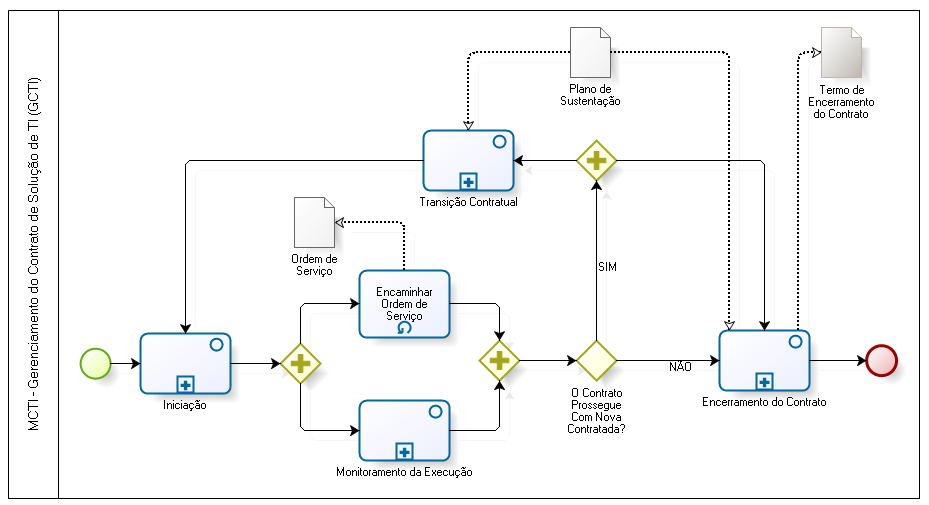
\includegraphics[scale=0.6]{figuras/GCTI.png}
		\caption{Gerenciamento de Contratações de Soluções de TI   \cite{mcti}}
\label{gcti}
\end{figure}



O encaminhamento formal de ordem de serviço ou fornecimento de bens pelo gestor do contrato para o preposto da contratada deve conter a definição e especificação dos serviços prestados ou bens fornecidos, o volume dos serviços ou quantidade de bens, segundo métricas, o cronograma e a identificação dos responsáveis pela solicitação da solução de TI. 

O monitoramento da execução consiste: na confecção e assinatura do termo de recebimento provisório, na avaliação da qualidade do serviço, na identificação de não conformidade, na verificação de aderência aos termos contratuais, na verificação da manutenção das condições classificatórias, no encaminhamento das demandas de correção à contratada ou de indicação de sanções, na confecção e assinatura do termo de recebimento definitivo, na autorização para emissão de nota fiscal, na verificação das regularidades fiscais, trabalhistas e previdenciárias, na verificação de manutenção de necessidade, economicidade e oportunidade da contratação, no encaminhamento de pedidos de modificação contratual e na manutenção do histórico de gerenciamento de contrato. 

E por fim, a etapa de transição contratual ou encerramento do contrato que deverá observar o Plano de Sustentação. Vale ressaltar que, para cada contrato, deverá haver pelo menos uma Ordem de Serviço ou de Fornecimento de Bens e pode haver quantas forem necessárias para execução do objeto contratado.

\section[Considerações Finais do Capítulo]{Considerações Finais do Capítulo}

Foi apresentado neste capítulo as principais referências legais no que diz respeito a contratação de fornecedores de desenvolvimento de \textit{software}. Este trabalho terá como foco a fase de Gerenciamento do Contrato do Modelo de Contratações de Soluções de TI. O gestor do contrato é o facilitador entre a parte negocial e a parte contratada. A forma ou metodologia de gestão de um contrato é um dos principais fatores que influenciam no sucesso do mesmo. O gerenciamento adequado dos contratos pode diminuir os riscos, promover mais rapidez, garantir conformidade com as necessidades negociais e garantir o controle e transparência sobre o que está sendo desenvolvido. Neste trabalho será analisada uma solução utilizada na Gestão de Contrato de uma organização pública brasileira que foi baseada no Pensamento Lean e em Metodologias Ágeis. O próximo capítulo irá caracterizar o Pensamento \textit{Lean}.

